% Created by tikzDevice version 0.12.3.1 on 2023-03-16 10:40:14
% !TEX encoding = UTF-8 Unicode
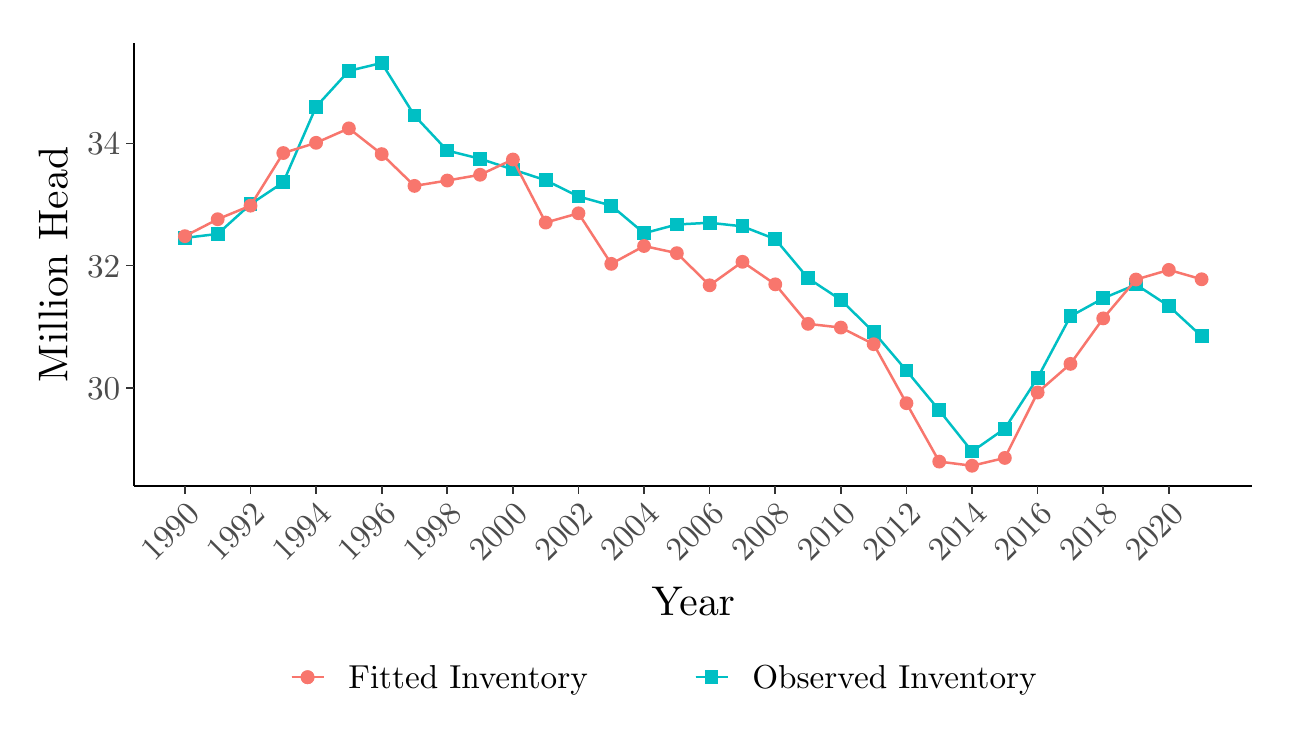
\begin{tikzpicture}[x=1pt,y=1pt]
\definecolor{fillColor}{RGB}{255,255,255}
\path[use as bounding box,fill=fillColor,fill opacity=0.00] (0,0) rectangle (448.07,252.94);
\begin{scope}
\path[clip] (  0.00,  0.00) rectangle (448.07,252.94);
\definecolor{drawColor}{RGB}{255,255,255}
\definecolor{fillColor}{RGB}{255,255,255}

\path[draw=drawColor,line width= 0.6pt,line join=round,line cap=round,fill=fillColor] (  0.00,  0.00) rectangle (448.07,252.94);
\end{scope}
\begin{scope}
\path[clip] ( 38.44, 87.36) rectangle (442.57,247.45);
\definecolor{fillColor}{RGB}{255,255,255}

\path[fill=fillColor] ( 38.44, 87.36) rectangle (442.57,247.44);
\definecolor{drawColor}{RGB}{0,191,196}

\path[draw=drawColor,line width= 0.9pt,line join=round] ( 56.81,176.97) --
	( 68.66,178.41) --
	( 80.52,189.15) --
	( 92.37,197.06) --
	(104.22,224.37) --
	(116.07,237.34) --
	(127.92,240.17) --
	(139.77,221.17) --
	(151.62,208.53) --
	(163.48,205.56) --
	(175.33,201.69) --
	(187.18,197.79) --
	(199.03,191.95) --
	(210.88,188.64) --
	(222.73,178.66) --
	(234.58,181.82) --
	(246.43,182.44) --
	(258.29,181.15) --
	(270.14,176.53) --
	(281.99,162.39) --
	(293.84,154.58) --
	(305.69,142.94) --
	(317.54,129.03) --
	(329.39,114.67) --
	(341.25, 99.78) --
	(353.10,108.07) --
	(364.95,126.42) --
	(376.80,148.64) --
	(388.65,155.16) --
	(400.50,160.11) --
	(412.35,152.35) --
	(424.20,141.42);
\definecolor{fillColor}{RGB}{0,191,196}

\path[fill=fillColor] ( 54.32,174.47) --
	( 59.31,174.47) --
	( 59.31,179.47) --
	( 54.32,179.47) --
	cycle;

\path[fill=fillColor] ( 66.17,175.91) --
	( 71.16,175.91) --
	( 71.16,180.91) --
	( 66.17,180.91) --
	cycle;

\path[fill=fillColor] ( 78.02,186.66) --
	( 83.01,186.66) --
	( 83.01,191.65) --
	( 78.02,191.65) --
	cycle;

\path[fill=fillColor] ( 89.87,194.56) --
	( 94.86,194.56) --
	( 94.86,199.55) --
	( 89.87,199.55) --
	cycle;

\path[fill=fillColor] (101.72,221.88) --
	(106.72,221.88) --
	(106.72,226.87) --
	(101.72,226.87) --
	cycle;

\path[fill=fillColor] (113.57,234.84) --
	(118.57,234.84) --
	(118.57,239.83) --
	(113.57,239.83) --
	cycle;

\path[fill=fillColor] (125.42,237.67) --
	(130.42,237.67) --
	(130.42,242.67) --
	(125.42,242.67) --
	cycle;

\path[fill=fillColor] (137.28,218.68) --
	(142.27,218.68) --
	(142.27,223.67) --
	(137.28,223.67) --
	cycle;

\path[fill=fillColor] (149.13,206.04) --
	(154.12,206.04) --
	(154.12,211.03) --
	(149.13,211.03) --
	cycle;

\path[fill=fillColor] (160.98,203.06) --
	(165.97,203.06) --
	(165.97,208.06) --
	(160.98,208.06) --
	cycle;

\path[fill=fillColor] (172.83,199.19) --
	(177.82,199.19) --
	(177.82,204.19) --
	(172.83,204.19) --
	cycle;

\path[fill=fillColor] (184.68,195.29) --
	(189.68,195.29) --
	(189.68,200.29) --
	(184.68,200.29) --
	cycle;

\path[fill=fillColor] (196.53,189.46) --
	(201.53,189.46) --
	(201.53,194.45) --
	(196.53,194.45) --
	cycle;

\path[fill=fillColor] (208.38,186.14) --
	(213.38,186.14) --
	(213.38,191.13) --
	(208.38,191.13) --
	cycle;

\path[fill=fillColor] (220.23,176.16) --
	(225.23,176.16) --
	(225.23,181.16) --
	(220.23,181.16) --
	cycle;

\path[fill=fillColor] (232.09,179.32) --
	(237.08,179.32) --
	(237.08,184.32) --
	(232.09,184.32) --
	cycle;

\path[fill=fillColor] (243.94,179.94) --
	(248.93,179.94) --
	(248.93,184.94) --
	(243.94,184.94) --
	cycle;

\path[fill=fillColor] (255.79,178.66) --
	(260.78,178.66) --
	(260.78,183.65) --
	(255.79,183.65) --
	cycle;

\path[fill=fillColor] (267.64,174.03) --
	(272.63,174.03) --
	(272.63,179.02) --
	(267.64,179.02) --
	cycle;

\path[fill=fillColor] (279.49,159.89) --
	(284.49,159.89) --
	(284.49,164.89) --
	(279.49,164.89) --
	cycle;

\path[fill=fillColor] (291.34,152.08) --
	(296.34,152.08) --
	(296.34,157.08) --
	(291.34,157.08) --
	cycle;

\path[fill=fillColor] (303.19,140.45) --
	(308.19,140.45) --
	(308.19,145.44) --
	(303.19,145.44) --
	cycle;

\path[fill=fillColor] (315.04,126.53) --
	(320.04,126.53) --
	(320.04,131.52) --
	(315.04,131.52) --
	cycle;

\path[fill=fillColor] (326.90,112.17) --
	(331.89,112.17) --
	(331.89,117.17) --
	(326.90,117.17) --
	cycle;

\path[fill=fillColor] (338.75, 97.28) --
	(343.74, 97.28) --
	(343.74,102.28) --
	(338.75,102.28) --
	cycle;

\path[fill=fillColor] (350.60,105.57) --
	(355.59,105.57) --
	(355.59,110.57) --
	(350.60,110.57) --
	cycle;

\path[fill=fillColor] (362.45,123.92) --
	(367.45,123.92) --
	(367.45,128.92) --
	(362.45,128.92) --
	cycle;

\path[fill=fillColor] (374.30,146.14) --
	(379.30,146.14) --
	(379.30,151.14) --
	(374.30,151.14) --
	cycle;

\path[fill=fillColor] (386.15,152.66) --
	(391.15,152.66) --
	(391.15,157.66) --
	(386.15,157.66) --
	cycle;

\path[fill=fillColor] (398.00,157.62) --
	(403.00,157.62) --
	(403.00,162.61) --
	(398.00,162.61) --
	cycle;

\path[fill=fillColor] (409.86,149.85) --
	(414.85,149.85) --
	(414.85,154.84) --
	(409.86,154.84) --
	cycle;

\path[fill=fillColor] (421.71,138.92) --
	(426.70,138.92) --
	(426.70,143.92) --
	(421.71,143.92) --
	cycle;
\definecolor{drawColor}{RGB}{248,118,109}

\path[draw=drawColor,line width= 0.9pt,line join=round] ( 56.81,177.60) --
	( 68.66,183.72) --
	( 80.52,188.62) --
	( 92.37,207.64) --
	(104.22,211.33) --
	(116.07,216.55) --
	(127.92,207.25) --
	(139.77,195.76) --
	(151.62,197.70) --
	(163.48,199.79) --
	(175.33,205.30) --
	(187.18,182.51) --
	(199.03,185.87) --
	(210.88,167.59) --
	(222.73,174.04) --
	(234.58,171.46) --
	(246.43,159.84) --
	(258.29,168.33) --
	(270.14,160.19) --
	(281.99,145.91) --
	(293.84,144.57) --
	(305.69,138.56) --
	(317.54,117.24) --
	(329.39, 96.14) --
	(341.25, 94.64) --
	(353.10, 97.47) --
	(364.95,121.12) --
	(376.80,131.45) --
	(388.65,147.89) --
	(400.50,161.93) --
	(412.35,165.41) --
	(424.20,162.02);
\definecolor{fillColor}{RGB}{248,118,109}

\path[fill=fillColor] ( 56.81,177.60) circle (  2.50);

\path[fill=fillColor] ( 68.66,183.72) circle (  2.50);

\path[fill=fillColor] ( 80.52,188.62) circle (  2.50);

\path[fill=fillColor] ( 92.37,207.64) circle (  2.50);

\path[fill=fillColor] (104.22,211.33) circle (  2.50);

\path[fill=fillColor] (116.07,216.55) circle (  2.50);

\path[fill=fillColor] (127.92,207.25) circle (  2.50);

\path[fill=fillColor] (139.77,195.76) circle (  2.50);

\path[fill=fillColor] (151.62,197.70) circle (  2.50);

\path[fill=fillColor] (163.48,199.79) circle (  2.50);

\path[fill=fillColor] (175.33,205.30) circle (  2.50);

\path[fill=fillColor] (187.18,182.51) circle (  2.50);

\path[fill=fillColor] (199.03,185.87) circle (  2.50);

\path[fill=fillColor] (210.88,167.59) circle (  2.50);

\path[fill=fillColor] (222.73,174.04) circle (  2.50);

\path[fill=fillColor] (234.58,171.46) circle (  2.50);

\path[fill=fillColor] (246.43,159.84) circle (  2.50);

\path[fill=fillColor] (258.29,168.33) circle (  2.50);

\path[fill=fillColor] (270.14,160.19) circle (  2.50);

\path[fill=fillColor] (281.99,145.91) circle (  2.50);

\path[fill=fillColor] (293.84,144.57) circle (  2.50);

\path[fill=fillColor] (305.69,138.56) circle (  2.50);

\path[fill=fillColor] (317.54,117.24) circle (  2.50);

\path[fill=fillColor] (329.39, 96.14) circle (  2.50);

\path[fill=fillColor] (341.25, 94.64) circle (  2.50);

\path[fill=fillColor] (353.10, 97.47) circle (  2.50);

\path[fill=fillColor] (364.95,121.12) circle (  2.50);

\path[fill=fillColor] (376.80,131.45) circle (  2.50);

\path[fill=fillColor] (388.65,147.89) circle (  2.50);

\path[fill=fillColor] (400.50,161.93) circle (  2.50);

\path[fill=fillColor] (412.35,165.41) circle (  2.50);

\path[fill=fillColor] (424.20,162.02) circle (  2.50);
\end{scope}
\begin{scope}
\path[clip] (  0.00,  0.00) rectangle (448.07,252.94);
\definecolor{drawColor}{RGB}{0,0,0}

\path[draw=drawColor,line width= 0.6pt,line join=round] ( 38.44, 87.36) --
	( 38.44,247.45);
\end{scope}
\begin{scope}
\path[clip] (  0.00,  0.00) rectangle (448.07,252.94);
\definecolor{drawColor}{gray}{0.30}

\node[text=drawColor,anchor=base east,inner sep=0pt, outer sep=0pt, scale=  1.20] at ( 33.49,118.67) {30};

\node[text=drawColor,anchor=base east,inner sep=0pt, outer sep=0pt, scale=  1.20] at ( 33.49,162.81) {32};

\node[text=drawColor,anchor=base east,inner sep=0pt, outer sep=0pt, scale=  1.20] at ( 33.49,206.94) {34};
\end{scope}
\begin{scope}
\path[clip] (  0.00,  0.00) rectangle (448.07,252.94);
\definecolor{drawColor}{gray}{0.20}

\path[draw=drawColor,line width= 0.6pt,line join=round] ( 35.69,122.81) --
	( 38.44,122.81);

\path[draw=drawColor,line width= 0.6pt,line join=round] ( 35.69,166.94) --
	( 38.44,166.94);

\path[draw=drawColor,line width= 0.6pt,line join=round] ( 35.69,211.07) --
	( 38.44,211.07);
\end{scope}
\begin{scope}
\path[clip] (  0.00,  0.00) rectangle (448.07,252.94);
\definecolor{drawColor}{RGB}{0,0,0}

\path[draw=drawColor,line width= 0.6pt,line join=round] ( 38.44, 87.36) --
	(442.57, 87.36);
\end{scope}
\begin{scope}
\path[clip] (  0.00,  0.00) rectangle (448.07,252.94);
\definecolor{drawColor}{gray}{0.20}

\path[draw=drawColor,line width= 0.6pt,line join=round] ( 56.81, 84.61) --
	( 56.81, 87.36);

\path[draw=drawColor,line width= 0.6pt,line join=round] ( 80.52, 84.61) --
	( 80.52, 87.36);

\path[draw=drawColor,line width= 0.6pt,line join=round] (104.22, 84.61) --
	(104.22, 87.36);

\path[draw=drawColor,line width= 0.6pt,line join=round] (127.92, 84.61) --
	(127.92, 87.36);

\path[draw=drawColor,line width= 0.6pt,line join=round] (151.62, 84.61) --
	(151.62, 87.36);

\path[draw=drawColor,line width= 0.6pt,line join=round] (175.33, 84.61) --
	(175.33, 87.36);

\path[draw=drawColor,line width= 0.6pt,line join=round] (199.03, 84.61) --
	(199.03, 87.36);

\path[draw=drawColor,line width= 0.6pt,line join=round] (222.73, 84.61) --
	(222.73, 87.36);

\path[draw=drawColor,line width= 0.6pt,line join=round] (246.43, 84.61) --
	(246.43, 87.36);

\path[draw=drawColor,line width= 0.6pt,line join=round] (270.14, 84.61) --
	(270.14, 87.36);

\path[draw=drawColor,line width= 0.6pt,line join=round] (293.84, 84.61) --
	(293.84, 87.36);

\path[draw=drawColor,line width= 0.6pt,line join=round] (317.54, 84.61) --
	(317.54, 87.36);

\path[draw=drawColor,line width= 0.6pt,line join=round] (341.25, 84.61) --
	(341.25, 87.36);

\path[draw=drawColor,line width= 0.6pt,line join=round] (364.95, 84.61) --
	(364.95, 87.36);

\path[draw=drawColor,line width= 0.6pt,line join=round] (388.65, 84.61) --
	(388.65, 87.36);

\path[draw=drawColor,line width= 0.6pt,line join=round] (412.35, 84.61) --
	(412.35, 87.36);
\end{scope}
\begin{scope}
\path[clip] (  0.00,  0.00) rectangle (448.07,252.94);
\definecolor{drawColor}{gray}{0.30}

\node[text=drawColor,rotate= 45.00,anchor=base east,inner sep=0pt, outer sep=0pt, scale=  1.20] at ( 62.66, 76.57) {1990};

\node[text=drawColor,rotate= 45.00,anchor=base east,inner sep=0pt, outer sep=0pt, scale=  1.20] at ( 86.36, 76.57) {1992};

\node[text=drawColor,rotate= 45.00,anchor=base east,inner sep=0pt, outer sep=0pt, scale=  1.20] at (110.06, 76.57) {1994};

\node[text=drawColor,rotate= 45.00,anchor=base east,inner sep=0pt, outer sep=0pt, scale=  1.20] at (133.77, 76.57) {1996};

\node[text=drawColor,rotate= 45.00,anchor=base east,inner sep=0pt, outer sep=0pt, scale=  1.20] at (157.47, 76.57) {1998};

\node[text=drawColor,rotate= 45.00,anchor=base east,inner sep=0pt, outer sep=0pt, scale=  1.20] at (181.17, 76.57) {2000};

\node[text=drawColor,rotate= 45.00,anchor=base east,inner sep=0pt, outer sep=0pt, scale=  1.20] at (204.87, 76.57) {2002};

\node[text=drawColor,rotate= 45.00,anchor=base east,inner sep=0pt, outer sep=0pt, scale=  1.20] at (228.58, 76.57) {2004};

\node[text=drawColor,rotate= 45.00,anchor=base east,inner sep=0pt, outer sep=0pt, scale=  1.20] at (252.28, 76.57) {2006};

\node[text=drawColor,rotate= 45.00,anchor=base east,inner sep=0pt, outer sep=0pt, scale=  1.20] at (275.98, 76.57) {2008};

\node[text=drawColor,rotate= 45.00,anchor=base east,inner sep=0pt, outer sep=0pt, scale=  1.20] at (299.68, 76.57) {2010};

\node[text=drawColor,rotate= 45.00,anchor=base east,inner sep=0pt, outer sep=0pt, scale=  1.20] at (323.39, 76.57) {2012};

\node[text=drawColor,rotate= 45.00,anchor=base east,inner sep=0pt, outer sep=0pt, scale=  1.20] at (347.09, 76.57) {2014};

\node[text=drawColor,rotate= 45.00,anchor=base east,inner sep=0pt, outer sep=0pt, scale=  1.20] at (370.79, 76.57) {2016};

\node[text=drawColor,rotate= 45.00,anchor=base east,inner sep=0pt, outer sep=0pt, scale=  1.20] at (394.49, 76.57) {2018};

\node[text=drawColor,rotate= 45.00,anchor=base east,inner sep=0pt, outer sep=0pt, scale=  1.20] at (418.20, 76.57) {2020};
\end{scope}
\begin{scope}
\path[clip] (  0.00,  0.00) rectangle (448.07,252.94);
\definecolor{drawColor}{RGB}{0,0,0}

\node[text=drawColor,anchor=base,inner sep=0pt, outer sep=0pt, scale=  1.50] at (240.51, 40.50) {Year};
\end{scope}
\begin{scope}
\path[clip] (  0.00,  0.00) rectangle (448.07,252.94);
\definecolor{drawColor}{RGB}{0,0,0}

\node[text=drawColor,rotate= 90.00,anchor=base,inner sep=0pt, outer sep=0pt, scale=  1.50] at ( 14.37,167.40) {Million Head};
\end{scope}
\begin{scope}
\path[clip] (  0.00,  0.00) rectangle (448.07,252.94);
\definecolor{fillColor}{RGB}{255,255,255}

\path[fill=fillColor] ( 80.91,  5.50) rectangle (400.11, 30.95);
\end{scope}
\begin{scope}
\path[clip] (  0.00,  0.00) rectangle (448.07,252.94);
\definecolor{drawColor}{RGB}{248,118,109}

\path[draw=drawColor,line width= 0.9pt,line join=round] ( 95.36, 18.23) -- (106.92, 18.23);
\end{scope}
\begin{scope}
\path[clip] (  0.00,  0.00) rectangle (448.07,252.94);
\definecolor{fillColor}{RGB}{248,118,109}

\path[fill=fillColor] (101.14, 18.23) circle (  2.50);
\end{scope}
\begin{scope}
\path[clip] (  0.00,  0.00) rectangle (448.07,252.94);
\definecolor{drawColor}{RGB}{248,118,109}

\path[draw=drawColor,line width= 0.9pt,line join=round] ( 95.36, 18.23) -- (106.92, 18.23);
\end{scope}
\begin{scope}
\path[clip] (  0.00,  0.00) rectangle (448.07,252.94);
\definecolor{fillColor}{RGB}{248,118,109}

\path[fill=fillColor] (101.14, 18.23) circle (  2.50);
\end{scope}
\begin{scope}
\path[clip] (  0.00,  0.00) rectangle (448.07,252.94);
\definecolor{drawColor}{RGB}{0,191,196}

\path[draw=drawColor,line width= 0.9pt,line join=round] (241.32, 18.23) -- (252.89, 18.23);
\end{scope}
\begin{scope}
\path[clip] (  0.00,  0.00) rectangle (448.07,252.94);
\definecolor{fillColor}{RGB}{0,191,196}

\path[fill=fillColor] (244.61, 15.73) --
	(249.60, 15.73) --
	(249.60, 20.72) --
	(244.61, 20.72) --
	cycle;
\end{scope}
\begin{scope}
\path[clip] (  0.00,  0.00) rectangle (448.07,252.94);
\definecolor{drawColor}{RGB}{0,191,196}

\path[draw=drawColor,line width= 0.9pt,line join=round] (241.32, 18.23) -- (252.89, 18.23);
\end{scope}
\begin{scope}
\path[clip] (  0.00,  0.00) rectangle (448.07,252.94);
\definecolor{fillColor}{RGB}{0,191,196}

\path[fill=fillColor] (244.61, 15.73) --
	(249.60, 15.73) --
	(249.60, 20.72) --
	(244.61, 20.72) --
	cycle;
\end{scope}
\begin{scope}
\path[clip] (  0.00,  0.00) rectangle (448.07,252.94);
\definecolor{drawColor}{RGB}{0,0,0}

\node[text=drawColor,anchor=base west,inner sep=0pt, outer sep=0pt, scale=  1.20] at (115.87, 14.09) {Fitted Inventory};
\end{scope}
\begin{scope}
\path[clip] (  0.00,  0.00) rectangle (448.07,252.94);
\definecolor{drawColor}{RGB}{0,0,0}

\node[text=drawColor,anchor=base west,inner sep=0pt, outer sep=0pt, scale=  1.20] at (261.83, 14.09) {Observed Inventory};
\end{scope}
\end{tikzpicture}
